\documentclass[a4paper,14pt]{article}
\usepackage{extsizes}
\usepackage{amsmath}
\usepackage{amssymb}
\everymath{\displaystyle}
\usepackage{geometry}
\usepackage{fancyhdr}
\usepackage{multicol}
\usepackage{graphicx}
\usepackage[brazil]{babel}
\usepackage[shortlabels]{enumitem}
\usepackage{cancel}
\columnsep=2cm
\hoffset=0cm
\textwidth=8cm
\setlength{\columnseprule}{.1pt}
\setlength{\columnsep}{2cm}
\renewcommand{\headrulewidth}{0pt}
\geometry{top=1in, bottom=1in, left=0.7in, right=0.5in}

\pagestyle{fancy}
\fancyhf{}
\fancyfoot[C]{\thepage}

\begin{document}
	
	\noindent\textbf{8FMA27~-~Matemática} 
	
	\begin{center}Área de trapézios (Versão estudante)
	\end{center}
	
	
	\noindent\textbf{Nome:} \underline{\hspace{10cm}}
	\noindent\textbf{Data:} \underline{\hspace{4cm}}
	
	%\section*{Questões de Matemática}
	
	\begin{multicols}{2}
	    \begin{enumerate}
	    	\item Num trapézio, a base menor mede 20 cm e a base maior mede 35 cm. A altura do trapézio é 18 cm. Qual é a área desse trapézio? \\\\\\\\\\\\\\\\\\\\\\\\
	    	\item A base maior de um trapézio mede 17 m e a base menor mede 9 m. A altura é igual a diferença dessas duas medidas. Qual é a área do trapézio? \\\\\\\\\\\\\\\\\\\\\\\\
	    	\item Um trapézio isóceles (isto é, cujos lados não paralelos são congruentes) tem dois lados de medida 15 cm e bases de medidas 8 e 26 cm. Calcule a área desse trapézio. \\\\\\\\\\\\\\\\\\\\
	    	\item Uma pequena casa tem duas paredes retangulares e duas paredes trapezoidais, como indicado na figura a seguir.
	    	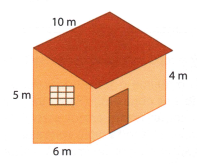
\includegraphics[width=1\linewidth]{8FMA27_imagens/pg146.png}\\
	    	São necessários 35 blocos para construir um metro quadrado dessas paredes. Sem considerar portas e janelas, calcule a quantidade de blocos utilizados na construção de todas as paredes da casa. \\\\\\\\\\\\\\\\\\\\
	    	\item O trapézio abaixo tem área igual s 63 cm² e altura igual a 7cm. Então a base maior e a base menor deste trapézio valem, respectivamente:
	    	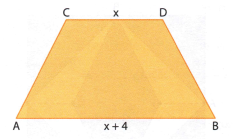
\includegraphics[width=1\linewidth]{8FMA27_imagens/pg158-1.png}\\
	    	\begin{enumerate}[a)]
	    		\item 11 cm e 7 cm.
	    		\item 12 cm e 8 cm.
	    		\item 9 cm e 5 cm.
	    		\item 7 cm e 3 cm.
	    		\item 21 cm e 17 cm. \\\\\\\\\\\\\\\\\\\\
	        \end{enumerate}
            \item Um trapézio tem área igual a 80, e uma de suas bases tem 6 unidades a mais do que a outra. Se a altura desse trapézio tem 5 unidades a mais do que a base menor, qual é a soma das medidas das bases e da altura?  \\\\\\\\\\\\\\\\\\\\
            \item O trapézio $ABCD$ tem m($A\hat{B}C$) = m($B\hat{C}D$) = 90$^\circ$, $AB = AD = 20$ m e $CD = $~36 m.
            \begin{enumerate}[a)]
            	\item Construa esse trapézio retângulo no Scratch (ou Snap!) Considere m($C\hat{D}A$) = 37$^\circ$ e 1 m = 10 passos.
            	\item Calcule a área do trapézio. \\\\\\\\\\\\\\\\\\\\
            \end{enumerate}
        	\item A área de um trapézio retângulo é 128 cm², e suas bases medem 19 cm e 13 cm. Determine o perímetro desse trapézio.
   	    \end{enumerate}
    \end{multicols}

\end{document}